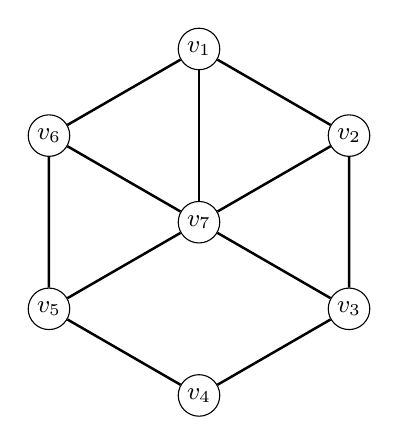
\begin{tikzpicture}[
  scale=1.0,
  vertex/.style={circle, draw=black, fill=white, inner sep=0pt, minimum size=15pt},
  every node/.style={font=\small}
]
  \node[vertex] (v1) at (90:2.2) {\(v_1\)};
  \node[vertex] (v2) at (30:2.2) {\(v_2\)};
  \node[vertex] (v3) at (-30:2.2) {\(v_3\)};
  \node[vertex] (v4) at (-90:2.2) {\(v_4\)};
  \node[vertex] (v5) at (-150:2.2) {\(v_5\)};
  \node[vertex] (v6) at (150:2.2) {\(v_6\)};
  \node[vertex] (v7) at (0,0) {\(v_7\)};

  \draw[line width=0.9pt] (v1) -- (v2) -- (v3) -- (v4) -- (v5) -- (v6) -- (v1);
  \draw[line width=0.9pt] (v7) -- (v1);
  \draw[line width=0.9pt] (v7) -- (v3);
  \draw[line width=0.9pt] (v7) -- (v5);
  \draw[line width=0.9pt] (v2) -- (v7);
  \draw[line width=0.9pt] (v6) -- (v7);

\end{tikzpicture}
